% Options for packages loaded elsewhere
\PassOptionsToPackage{unicode}{hyperref}
\PassOptionsToPackage{hyphens}{url}
\PassOptionsToPackage{dvipsnames,svgnames,x11names}{xcolor}
%
\documentclass[
  10pt,
  letterpaper,
  DIV=11,
  numbers=noendperiod]{scrartcl}

\usepackage{amsmath,amssymb}
\usepackage{setspace}
\usepackage{iftex}
\ifPDFTeX
  \usepackage[T1]{fontenc}
  \usepackage[utf8]{inputenc}
  \usepackage{textcomp} % provide euro and other symbols
\else % if luatex or xetex
  \usepackage{unicode-math}
  \defaultfontfeatures{Scale=MatchLowercase}
  \defaultfontfeatures[\rmfamily]{Ligatures=TeX,Scale=1}
\fi
\usepackage{lmodern}
\ifPDFTeX\else  
    % xetex/luatex font selection
\fi
% Use upquote if available, for straight quotes in verbatim environments
\IfFileExists{upquote.sty}{\usepackage{upquote}}{}
\IfFileExists{microtype.sty}{% use microtype if available
  \usepackage[]{microtype}
  \UseMicrotypeSet[protrusion]{basicmath} % disable protrusion for tt fonts
}{}
\usepackage{xcolor}
\usepackage[lmargin=0.5in,rmargin=0.5in,tmargin=0.5in,bmargin=0.5in]{geometry}
\setlength{\emergencystretch}{3em} % prevent overfull lines
\setcounter{secnumdepth}{-\maxdimen} % remove section numbering
% Make \paragraph and \subparagraph free-standing
\ifx\paragraph\undefined\else
  \let\oldparagraph\paragraph
  \renewcommand{\paragraph}[1]{\oldparagraph{#1}\mbox{}}
\fi
\ifx\subparagraph\undefined\else
  \let\oldsubparagraph\subparagraph
  \renewcommand{\subparagraph}[1]{\oldsubparagraph{#1}\mbox{}}
\fi


\providecommand{\tightlist}{%
  \setlength{\itemsep}{0pt}\setlength{\parskip}{0pt}}\usepackage{longtable,booktabs,array}
\usepackage{calc} % for calculating minipage widths
% Correct order of tables after \paragraph or \subparagraph
\usepackage{etoolbox}
\makeatletter
\patchcmd\longtable{\par}{\if@noskipsec\mbox{}\fi\par}{}{}
\makeatother
% Allow footnotes in longtable head/foot
\IfFileExists{footnotehyper.sty}{\usepackage{footnotehyper}}{\usepackage{footnote}}
\makesavenoteenv{longtable}
\usepackage{graphicx}
\makeatletter
\def\maxwidth{\ifdim\Gin@nat@width>\linewidth\linewidth\else\Gin@nat@width\fi}
\def\maxheight{\ifdim\Gin@nat@height>\textheight\textheight\else\Gin@nat@height\fi}
\makeatother
% Scale images if necessary, so that they will not overflow the page
% margins by default, and it is still possible to overwrite the defaults
% using explicit options in \includegraphics[width, height, ...]{}
\setkeys{Gin}{width=\maxwidth,height=\maxheight,keepaspectratio}
% Set default figure placement to htbp
\makeatletter
\def\fps@figure{htbp}
\makeatother

\usepackage[pages=some]{background}

\RedeclareSectionCommand[font=\centering\large]{section}
\RedeclareSectionCommand[
  runin=false,
  afterindent=false,
  font = \normalfont\textbf,
  beforeskip=0pt,
  afterskip=0pt]{subsection}

\setlength{\itemsep}{1pt}
\setlength{\parskip}{0pt}
\setlength{\parsep}{0pt}
\setlength{\labelsep}{0pt}
\setlength{\topsep}{0pt}
\setlength{\parsep}{0pt}
\setlength{\partopsep}{0pt}
\usepackage{fontspec}
\usepackage{multirow}
\usepackage{multicol}
\usepackage{colortbl}
\usepackage{hhline}
\newlength\Oldarrayrulewidth
\newlength\Oldtabcolsep
\usepackage{longtable}
\usepackage{array}
\usepackage{hyperref}
\usepackage{float}
\usepackage{wrapfig}
\KOMAoption{captions}{tableheading}
\makeatletter
\@ifpackageloaded{caption}{}{\usepackage{caption}}
\AtBeginDocument{%
\ifdefined\contentsname
  \renewcommand*\contentsname{Table of contents}
\else
  \newcommand\contentsname{Table of contents}
\fi
\ifdefined\listfigurename
  \renewcommand*\listfigurename{List of Figures}
\else
  \newcommand\listfigurename{List of Figures}
\fi
\ifdefined\listtablename
  \renewcommand*\listtablename{List of Tables}
\else
  \newcommand\listtablename{List of Tables}
\fi
\ifdefined\figurename
  \renewcommand*\figurename{Figure}
\else
  \newcommand\figurename{Figure}
\fi
\ifdefined\tablename
  \renewcommand*\tablename{Table}
\else
  \newcommand\tablename{Table}
\fi
}
\@ifpackageloaded{float}{}{\usepackage{float}}
\floatstyle{ruled}
\@ifundefined{c@chapter}{\newfloat{codelisting}{h}{lop}}{\newfloat{codelisting}{h}{lop}[chapter]}
\floatname{codelisting}{Listing}
\newcommand*\listoflistings{\listof{codelisting}{List of Listings}}
\makeatother
\makeatletter
\makeatother
\makeatletter
\@ifpackageloaded{caption}{}{\usepackage{caption}}
\@ifpackageloaded{subcaption}{}{\usepackage{subcaption}}
\makeatother
\ifLuaTeX
  \usepackage{selnolig}  % disable illegal ligatures
\fi
\usepackage{bookmark}

\IfFileExists{xurl.sty}{\usepackage{xurl}}{} % add URL line breaks if available
\urlstyle{same} % disable monospaced font for URLs
\hypersetup{
  pdftitle={Black Sea Bass () Ecosystem \& Socioeconomic Profile Report Card},
  colorlinks=true,
  linkcolor={blue},
  filecolor={Maroon},
  citecolor={Blue},
  urlcolor={Blue},
  pdfcreator={LaTeX via pandoc}}

\title{Black Sea Bass (\protect\textit{Centropristis striata})
\linebreak Ecosystem \& Socioeconomic Profile Report Card}
\author{}
\date{}

\begin{document}
\maketitle

\setstretch{1}
\backgroundsetup{
  scale=1,
  angle=0,
  opacity=0,
  contents={
\includegraphics[width=\paperwidth,height=\paperheight]{bg_pg1.jpg}}
 }
\BgThispage

\vspace{-2.5cm}
\section{Spring 2025}

This is a short-form update to the full Ecosystem and Socioeconomic
Profile (Tabandera et al., 2024) highlighting the recent status of
environmental, ecological, and socioeconomic factors. Black sea bass is
an important Mid-Atlantic stock with high commercial value and
recreational engagement. Overfishing is not occurring and the stock is
not overfished. Winter bottom temperature is used in the stock
assessment model as a factor that influences recruitment to incorporate
the observed link between cold temperature and smaller year classes
(NEFSC 2023).

\begin{figure}

\begin{minipage}{0.40\linewidth}
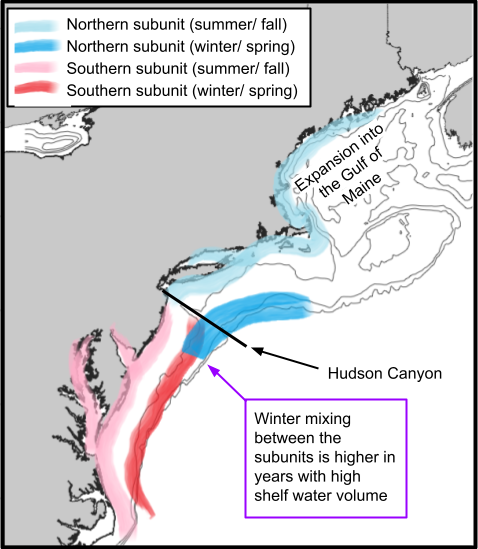
\includegraphics{C:/Users/abigail.tyrell/Documents/code/bsb/images/bsb spatiotemporal conceptual model.png}\end{minipage}%
%
\begin{minipage}{0.03\linewidth}

\hfill

\end{minipage}%
%
\begin{minipage}{0.57\linewidth}

\section{2024 in Review}

\subsection{Fishing Community Observations (MAFMC 2024a-c)}

\begin{itemize}
\tightlist
\item
  Steady or increasing availability
\item
  Restrictive and complex regulations limit fishing opportunities
\item
  Concerns about high discards
\end{itemize}

\vspace{-0.25cm}
\subsection{Commercial Fishery}

\begin{itemize}
\tightlist
\item
  Number of active vessels declined in 2024, but total landed pounds
  increased from 2023
\item
  Total revenue decreased slightly along with average prices (\$/lb)
\item
  Average revenue per vessel increased
\end{itemize}

\vspace{-0.25cm}
\subsection{Recreational Fishery}

\begin{itemize}
\tightlist
\item
  Number of targeted trips, catch, and landings all down from 2023
  (MAFMC 2024a)
\item
  However, number of trips is still above the historic average
\item
  Recreational catch-per-angler index not yet updated for 2024
\end{itemize}

\vspace{-0.25cm}
\subsection{Ecosystem}

\begin{itemize}
\tightlist
\item
  The stock assessment models the stock as two subunits, divided at the
  Hudson Canyon (see right)
\item
  Cold winter in the north but near average in the south
\item
  Poor or below average fish condition (i.e., weight at a given length)
  in recent years
\end{itemize}

\end{minipage}%
\newline
\begin{minipage}{\linewidth}

\vspace{0.25cm}
\section{Key Points from the Mid-Atlantic Risk Assessment}
\vspace{0.05cm}

\end{minipage}%
\newline
\begin{minipage}{0.57\linewidth}

\raggedright

According to the
\href{https://static1.squarespace.com/static/511cdc7fe4b00307a2628ac6/t/6747560a3cf66936045e5547/1732728332670/05_EAFM+Risk+Assessment.pdf}{Mid-Atlantic
2024 EAFM risk assessment update} (MAFMC 2024d), Black Sea Bass scored
high and/or moderately high risk in the following elements (elements
with low or low-moderate scores not described here):

\begin{itemize}
\tightlist
\item
  Moderate-high to high risk to the stock due to:

  \begin{itemize}
  \tightlist
  \item
    Very high exposure to changes in climate
  \item
    Observed and potential changes in distribution; northward shift into
    the Gulf of Maine
  \item
    Dependence on threatened estuarine habitat
  \item
    Decline in the biomass of benthic invertebrate prey
  \item
    Decline in black sea bass body condition
  \end{itemize}
\item
  High risk to the recreational fishery due to:

  \begin{itemize}
  \tightlist
  \item
    Catch exceeding harvest limits in several years
  \item
    High regulatory complexity; frequent changes and varying interstate
    regulations; regulatory changes in allocations
  \end{itemize}
\item
  Moderate-high risk to the commercial fishery due to:

  \begin{itemize}
  \tightlist
  \item
    Commercial revenue in wind development areas
  \item
    High discards \& discard mortality
  \end{itemize}
\end{itemize}

\end{minipage}%
%
\begin{minipage}{0.03\linewidth}

\hfill

\end{minipage}%
%
\begin{minipage}{0.40\linewidth}
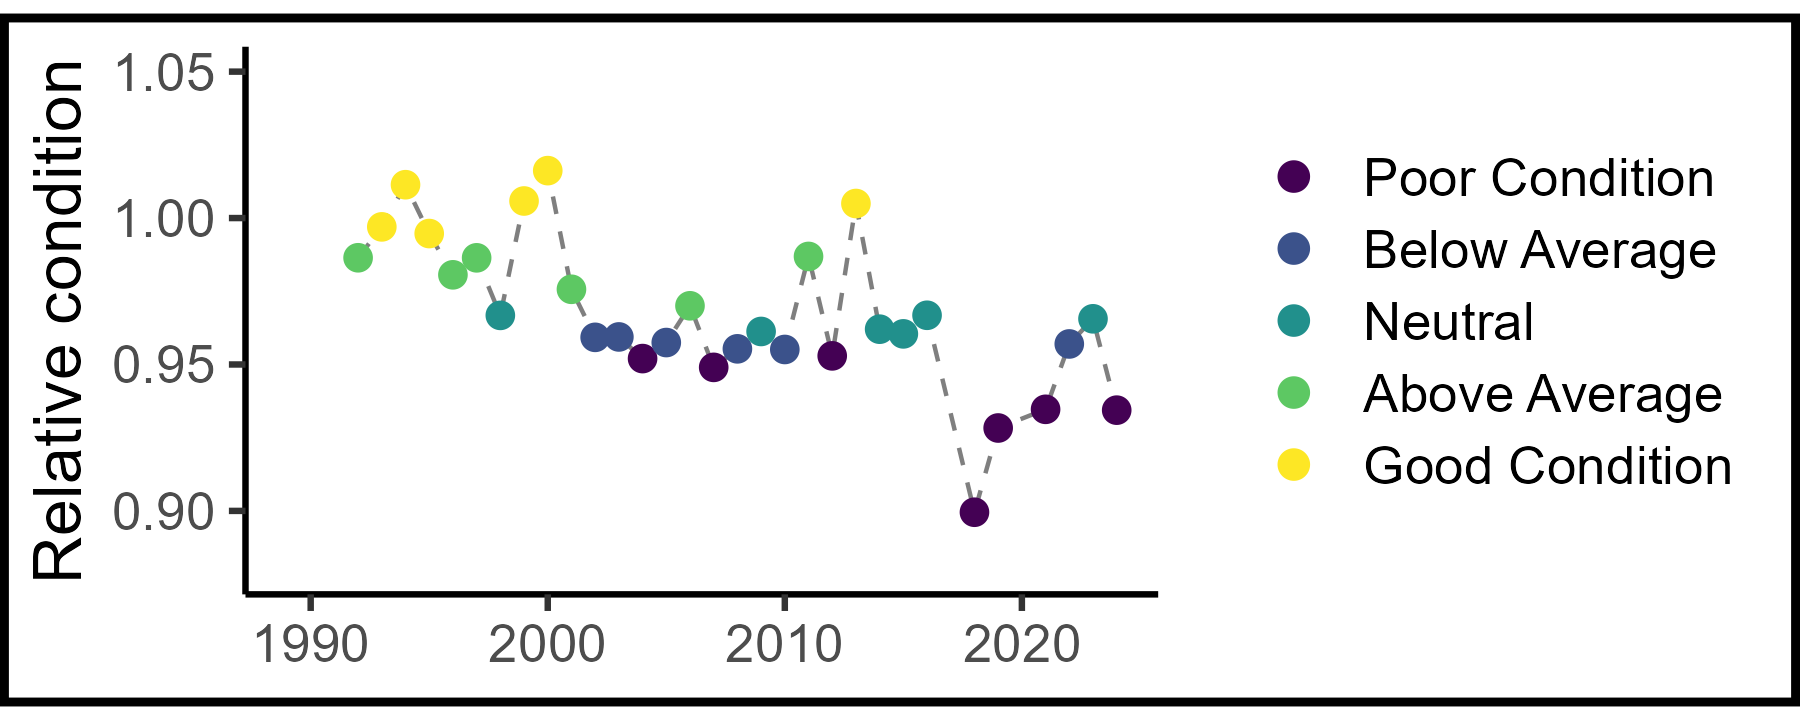
\includegraphics{C:/Users/abigail.tyrell/Documents/code/bsb/images/new_condition.png}
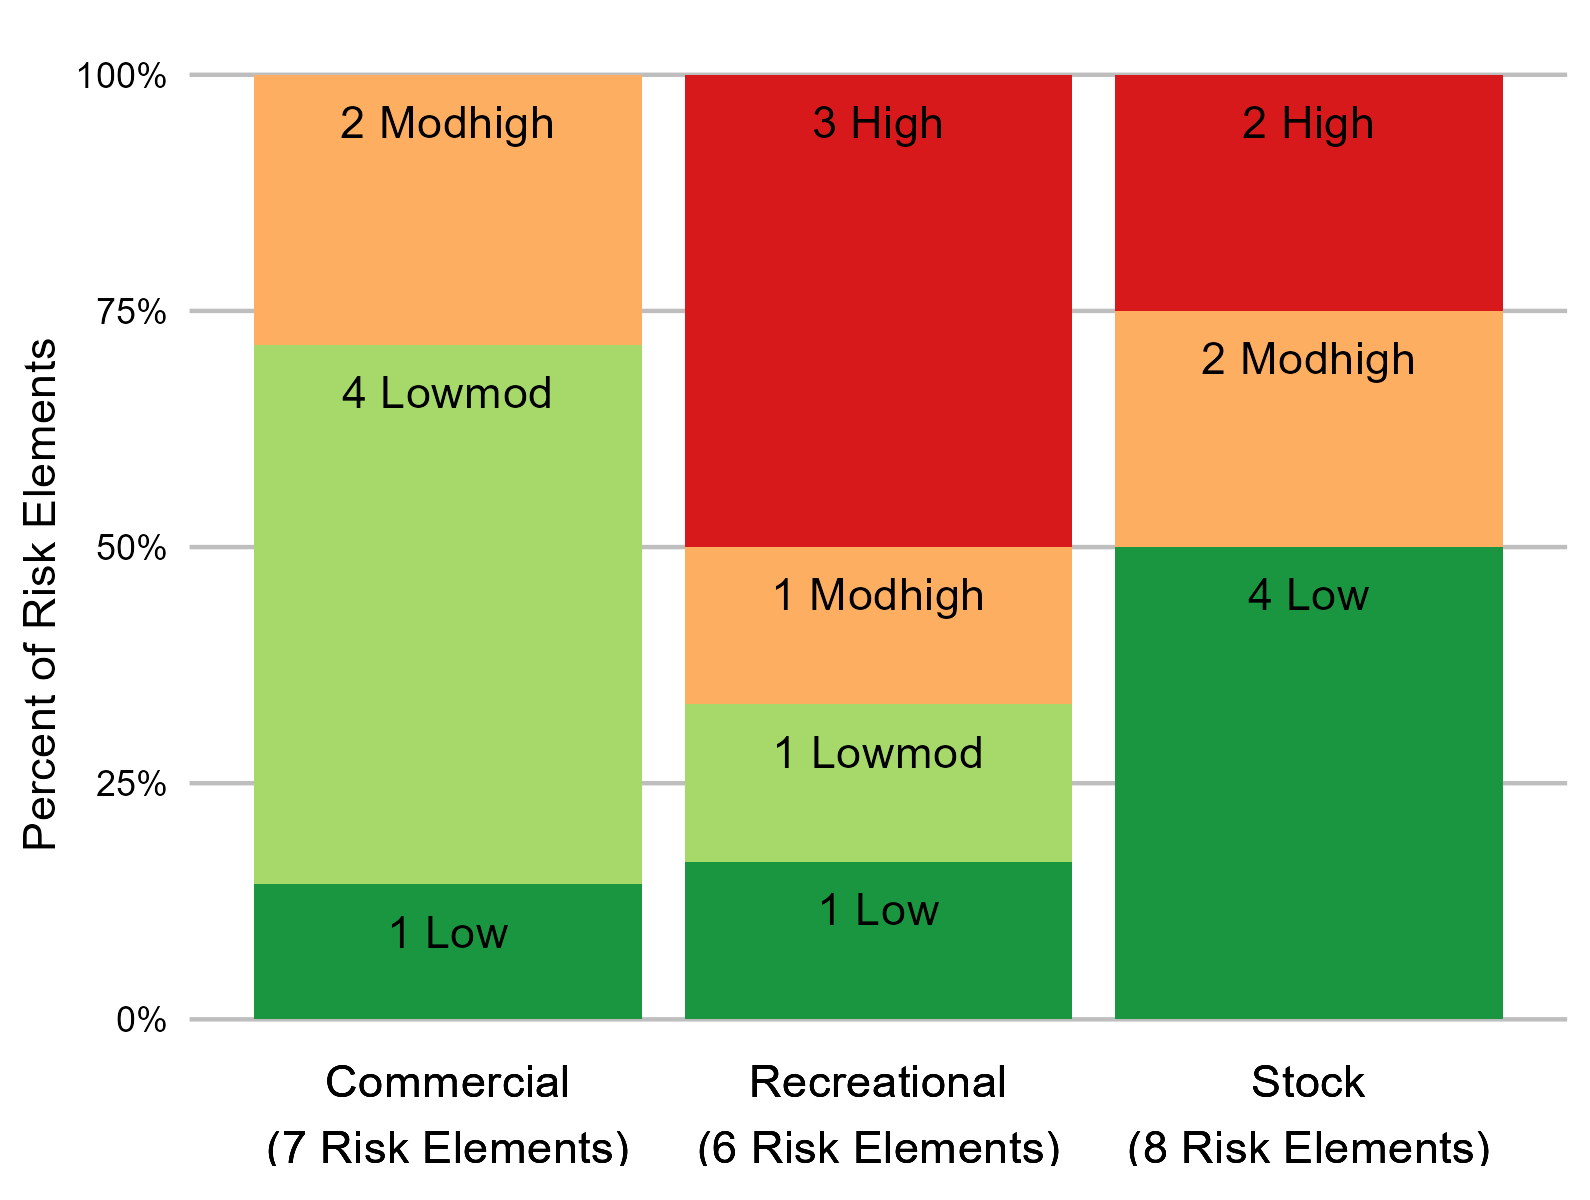
\includegraphics{C:/Users/abigail.tyrell/Documents/code/bsb/images/risk_plot.png}\end{minipage}%

\end{figure}%

\newpage

\backgroundsetup{
  scale=1,
  angle=0,
  opacity=0,
  contents={
\includegraphics[width=\paperwidth,height=\paperheight]{bg_pg2.jpg}}
 }
\BgThispage

\global\setlength{\Oldarrayrulewidth}{\arrayrulewidth}

\global\setlength{\Oldtabcolsep}{\tabcolsep}

\setlength{\tabcolsep}{2pt}

\renewcommand*{\arraystretch}{1.5}



\providecommand{\ascline}[3]{\noalign{\global\arrayrulewidth #1}\arrayrulecolor[HTML]{#2}\cline{#3}}

\begin{longtable*}[c]{|p{0.90in}|p{0.75in}|p{2.50in}|p{3.00in}}



\ascline{0.75pt}{666666}{1-4}

\multicolumn{1}{!{\color[HTML]{666666}\vrule width 0.75pt}>{\centering}m{\dimexpr 0.9in+0\tabcolsep}}{\textcolor[HTML]{000000}{\fontsize{10}{10}\selectfont{\global\setmainfont{Times New Roman}{\textbf{Indicator}}}}} & \multicolumn{1}{!{\color[HTML]{666666}\vrule width 0.75pt}>{\centering}m{\dimexpr 0.75in+0\tabcolsep}}{\textcolor[HTML]{000000}{\fontsize{10}{10}\selectfont{\global\setmainfont{Times New Roman}{\textbf{Status\ In\ }}}}} & \multicolumn{1}{!{\color[HTML]{666666}\vrule width 0.75pt}>{\centering}m{\dimexpr 2.5in+0\tabcolsep}}{\textcolor[HTML]{000000}{\fontsize{10}{10}\selectfont{\global\setmainfont{Times New Roman}{\textbf{Implications}}}}} & \multicolumn{1}{!{\color[HTML]{666666}\vrule width 0.75pt}>{\centering}m{\dimexpr 3in+0\tabcolsep}!{\color[HTML]{666666}\vrule width 0.75pt}}{\textcolor[HTML]{000000}{\fontsize{10}{10}\selectfont{\global\setmainfont{Times New Roman}{\textbf{Time\ Series*}}}}} \\

\ascline{0.75pt}{666666}{1-4}\endfirsthead 

\ascline{0.75pt}{666666}{1-4}

\multicolumn{1}{!{\color[HTML]{666666}\vrule width 0.75pt}>{\centering}m{\dimexpr 0.9in+0\tabcolsep}}{\textcolor[HTML]{000000}{\fontsize{10}{10}\selectfont{\global\setmainfont{Times New Roman}{\textbf{Indicator}}}}} & \multicolumn{1}{!{\color[HTML]{666666}\vrule width 0.75pt}>{\centering}m{\dimexpr 0.75in+0\tabcolsep}}{\textcolor[HTML]{000000}{\fontsize{10}{10}\selectfont{\global\setmainfont{Times New Roman}{\textbf{Status\ In\ }}}}} & \multicolumn{1}{!{\color[HTML]{666666}\vrule width 0.75pt}>{\centering}m{\dimexpr 2.5in+0\tabcolsep}}{\textcolor[HTML]{000000}{\fontsize{10}{10}\selectfont{\global\setmainfont{Times New Roman}{\textbf{Implications}}}}} & \multicolumn{1}{!{\color[HTML]{666666}\vrule width 0.75pt}>{\centering}m{\dimexpr 3in+0\tabcolsep}!{\color[HTML]{666666}\vrule width 0.75pt}}{\textcolor[HTML]{000000}{\fontsize{10}{10}\selectfont{\global\setmainfont{Times New Roman}{\textbf{Time\ Series*}}}}} \\

\ascline{0.75pt}{666666}{1-4}\endhead



\multicolumn{1}{!{\color[HTML]{666666}\vrule width 0.75pt}>{\raggedright}m{\dimexpr 0.9in+0\tabcolsep}}{\textcolor[HTML]{000000}{\fontsize{10}{10}\selectfont{\global\setmainfont{Times New Roman}{Mean\ winter\ (Feb-Mar)\ bottom\ temperature\ (C)}}}} & \multicolumn{1}{!{\color[HTML]{666666}\vrule width 0.75pt}>{\raggedright}m{\dimexpr 0.75in+0\tabcolsep}}{\textcolor[HTML]{000000}{\fontsize{10}{10}\selectfont{\global\setmainfont{Times New Roman}{North:\ Below\ threshold\ South:\ Near\ long-term\ average}}}} & \multicolumn{1}{!{\color[HTML]{666666}\vrule width 0.75pt}>{\raggedright}m{\dimexpr 2.5in+0\tabcolsep}}{\textcolor[HTML]{000000}{\fontsize{10}{10}\selectfont{\global\setmainfont{Times New Roman}{Cold\ winter\ temperatures\ may\ increase\ the\ mortality\ of\ young-of-the-year\ fish,\ resulting\ in\ smaller\ year\ classes.\ 2024\ temperature\ in\ the\ northern\ subunit\ (north\ of\ Hudson\ Canyon)\ was\ colder\ than\ black\ sea\ bass's\ lower\ threshold\ of\ 8C.\ Bottom\ temperature\ data\ comes\ from\ GLORYS,\ a\ modeled\ product\ (Jean-Michel\ et\ al.,\ 2021).}}}} & \multicolumn{1}{!{\color[HTML]{666666}\vrule width 0.75pt}>{\centering}m{\dimexpr 3in+0\tabcolsep}!{\color[HTML]{666666}\vrule width 0.75pt}}{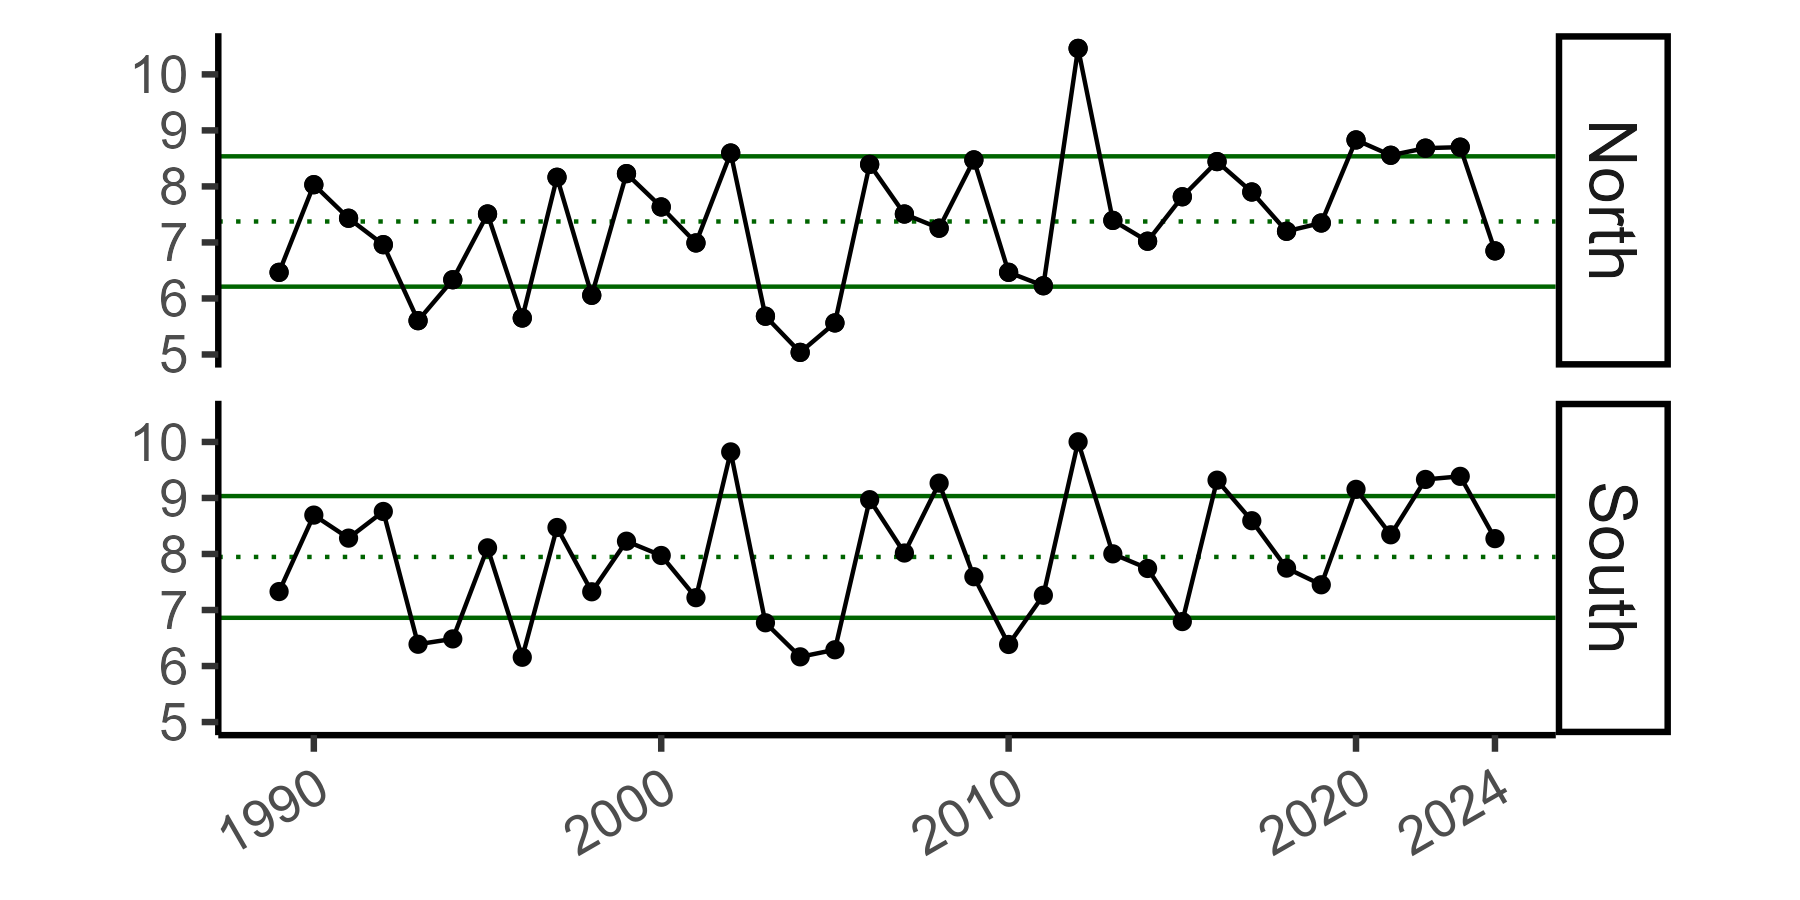
\includegraphics[width=3in, height=1.5in]{bsb_report_card_files/figure-pdf/unnamed-chunk-4-1.png}} \\

\ascline{0.75pt}{666666}{1-4}



\multicolumn{1}{!{\color[HTML]{666666}\vrule width 0.75pt}>{\raggedright}m{\dimexpr 0.9in+0\tabcolsep}}{\textcolor[HTML]{000000}{\fontsize{10}{10}\selectfont{\global\setmainfont{Times New Roman}{Shelf\ water\ volume\ (km3)}}}} & \multicolumn{1}{!{\color[HTML]{666666}\vrule width 0.75pt}>{\raggedright}m{\dimexpr 0.75in+0\tabcolsep}}{\textcolor[HTML]{000000}{\fontsize{10}{10}\selectfont{\global\setmainfont{Times New Roman}{No\ data\ for\ 2024}}}} & \multicolumn{1}{!{\color[HTML]{666666}\vrule width 0.75pt}>{\raggedright}m{\dimexpr 2.5in+0\tabcolsep}}{\textcolor[HTML]{000000}{\fontsize{10}{10}\selectfont{\global\setmainfont{Times New Roman}{Shelf\ water\ volume\ (Fratantoni\ et\ al.,\ 2015)\ is\ a\ proxy\ for\ suitable\ winter\ habitat;\ higher\ shelf\ water\ volume\ indicates\ less\ suitable\ habitat,\ potentially\ leading\ to\ northern\ fish\ migrating\ into\ the\ southern\ subunit.\ The\ shelf\ water\ volume\ dataset\ is\ created\ from\ in\ situ\ data,\ and\ there\ has\ been\ no\ winter\ sampling\ since\ 2021,\ highlighting\ the\ need\ for\ additional\ indicators\ to\ inform\ stock\ subunit\ mixing.}}}} & \multicolumn{1}{!{\color[HTML]{666666}\vrule width 0.75pt}>{\centering}m{\dimexpr 3in+0\tabcolsep}!{\color[HTML]{666666}\vrule width 0.75pt}}{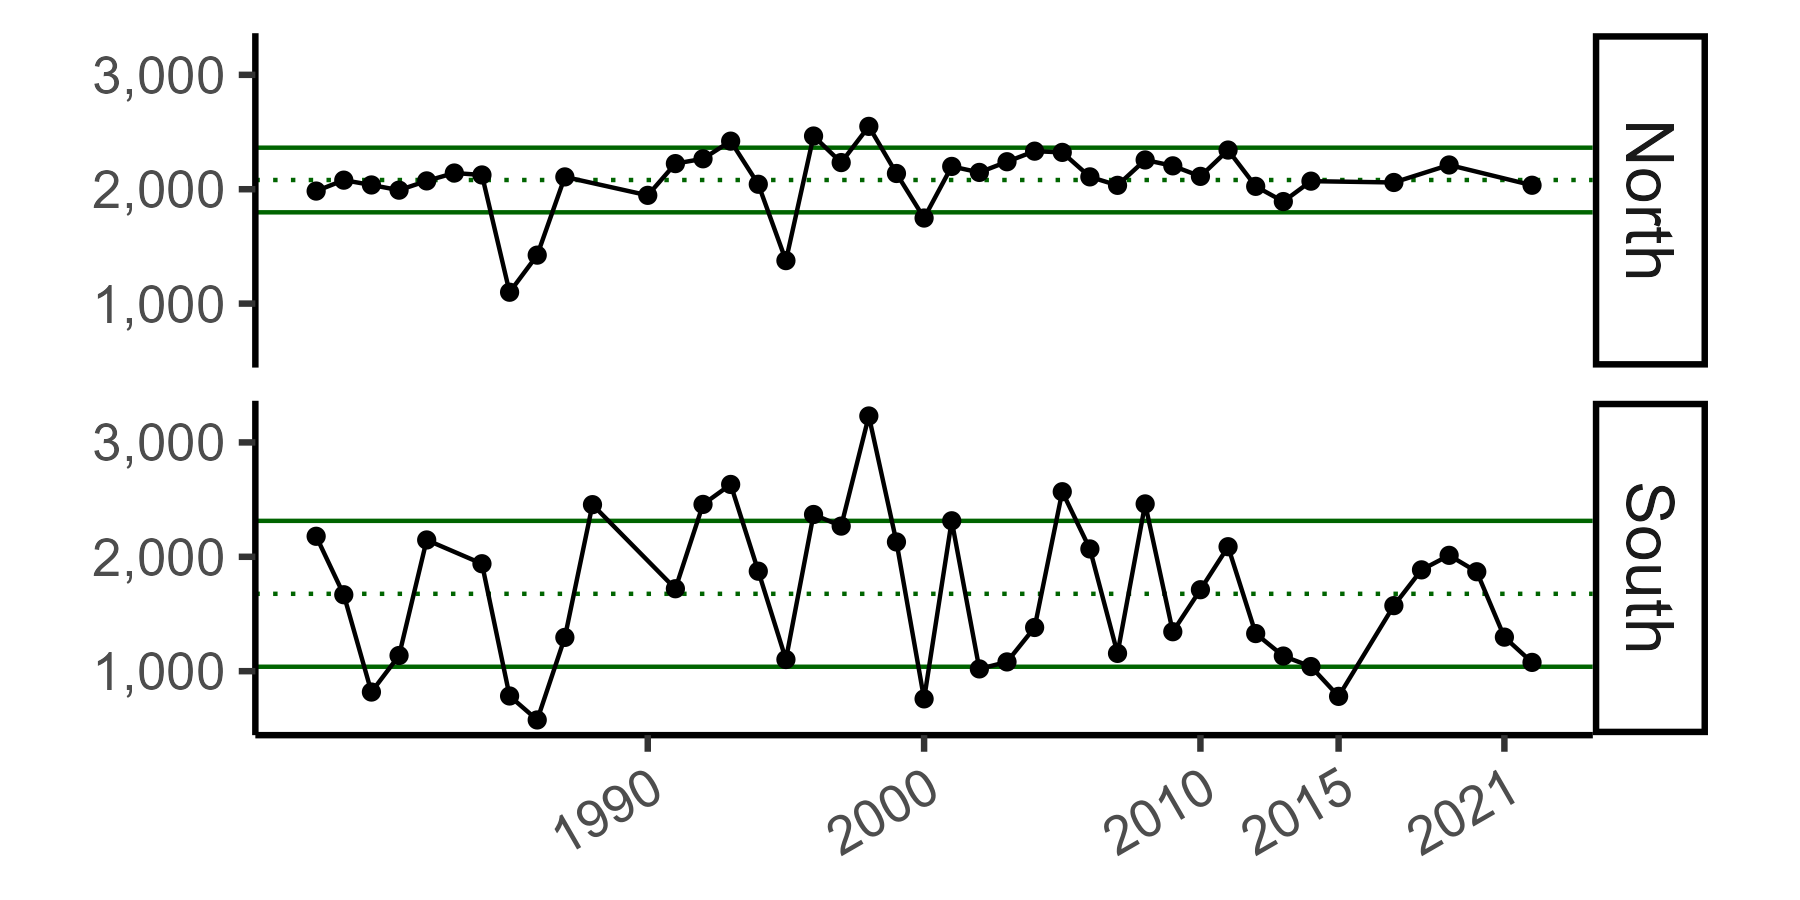
\includegraphics[width=3in, height=1.5in]{bsb_report_card_files/figure-pdf/unnamed-chunk-4-2.png}} \\

\ascline{0.75pt}{666666}{1-4}



\multicolumn{1}{!{\color[HTML]{666666}\vrule width 0.75pt}>{\raggedright}m{\dimexpr 0.9in+0\tabcolsep}}{\textcolor[HTML]{000000}{\fontsize{10}{10}\selectfont{\global\setmainfont{Times New Roman}{Black\ sea\ bass\ MRIP\ recreational\ trips\ (millions\ of\ annual\ trips)}}}} & \multicolumn{1}{!{\color[HTML]{666666}\vrule width 0.75pt}>{\raggedright}m{\dimexpr 0.75in+0\tabcolsep}}{\textcolor[HTML]{000000}{\fontsize{10}{10}\selectfont{\global\setmainfont{Times New Roman}{Above\ long-term\ average}}}} & \multicolumn{1}{!{\color[HTML]{666666}\vrule width 0.75pt}>{\raggedright}m{\dimexpr 2.5in+0\tabcolsep}}{\textcolor[HTML]{000000}{\fontsize{10}{10}\selectfont{\global\setmainfont{Times New Roman}{Recent\ trip\ numbers\ are\ near\ an\ all-time\ high,\ but\ have\ decreased\ from\ 2023.\ Catch\ (not\ shown)\ generally\ reflects\ trip\ patterns,\ while\ landings\ (not\ shown)\ have\ remained\ steady.\ High\ regulatory\ complexity\ is\ likely\ contributing\ to\ recreational\ fishing\ trends.}}}} & \multicolumn{1}{!{\color[HTML]{666666}\vrule width 0.75pt}>{\centering}m{\dimexpr 3in+0\tabcolsep}!{\color[HTML]{666666}\vrule width 0.75pt}}{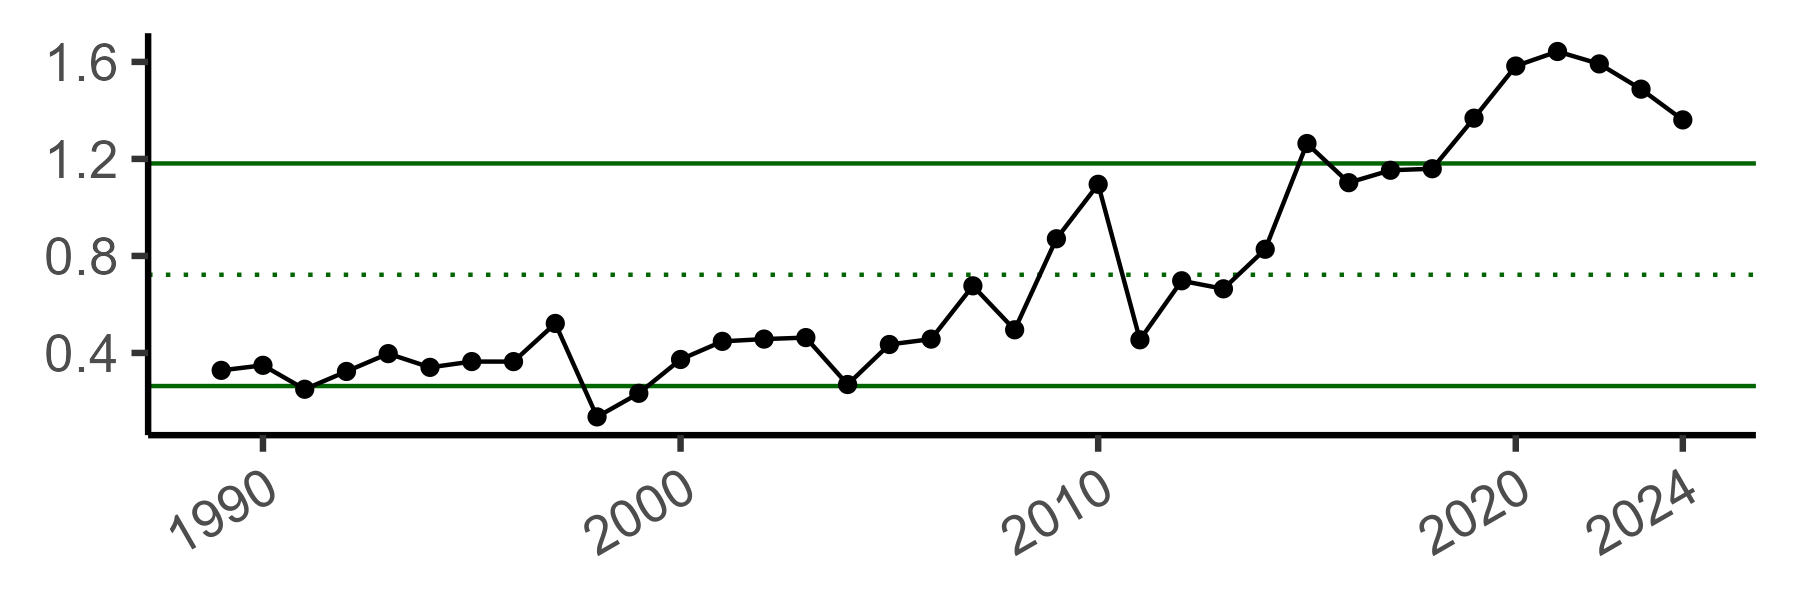
\includegraphics[width=3in, height=1in]{bsb_report_card_files/figure-pdf/unnamed-chunk-4-3.png}} \\

\ascline{0.75pt}{666666}{1-4}



\multicolumn{1}{!{\color[HTML]{666666}\vrule width 0.75pt}>{\raggedright}m{\dimexpr 0.9in+0\tabcolsep}}{\textcolor[HTML]{000000}{\fontsize{10}{10}\selectfont{\global\setmainfont{Times New Roman}{Commercial\ revenue\ per\ vessel\ (2024\ USD)}}}} & \multicolumn{1}{!{\color[HTML]{666666}\vrule width 0.75pt}>{\raggedright}m{\dimexpr 0.75in+0\tabcolsep}}{\textcolor[HTML]{000000}{\fontsize{10}{10}\selectfont{\global\setmainfont{Times New Roman}{Above\ long-term\ average}}}} & \multicolumn{1}{!{\color[HTML]{666666}\vrule width 0.75pt}>{\raggedright}m{\dimexpr 2.5in+0\tabcolsep}}{\textcolor[HTML]{000000}{\fontsize{10}{10}\selectfont{\global\setmainfont{Times New Roman}{Commercial\ revenue\ per\ vessel\ follows\ an\ overall\ increasing\ trend\ most\ likely\ driven\ by\ the\ continued\ decline\ of\ active\ vessels\ and\ an\ overall\ increase\ in\ total\ commercial\ landed\ pounds\ over\ the\ past\ decade.\  \ }}}} & \multicolumn{1}{!{\color[HTML]{666666}\vrule width 0.75pt}>{\centering}m{\dimexpr 3in+0\tabcolsep}!{\color[HTML]{666666}\vrule width 0.75pt}}{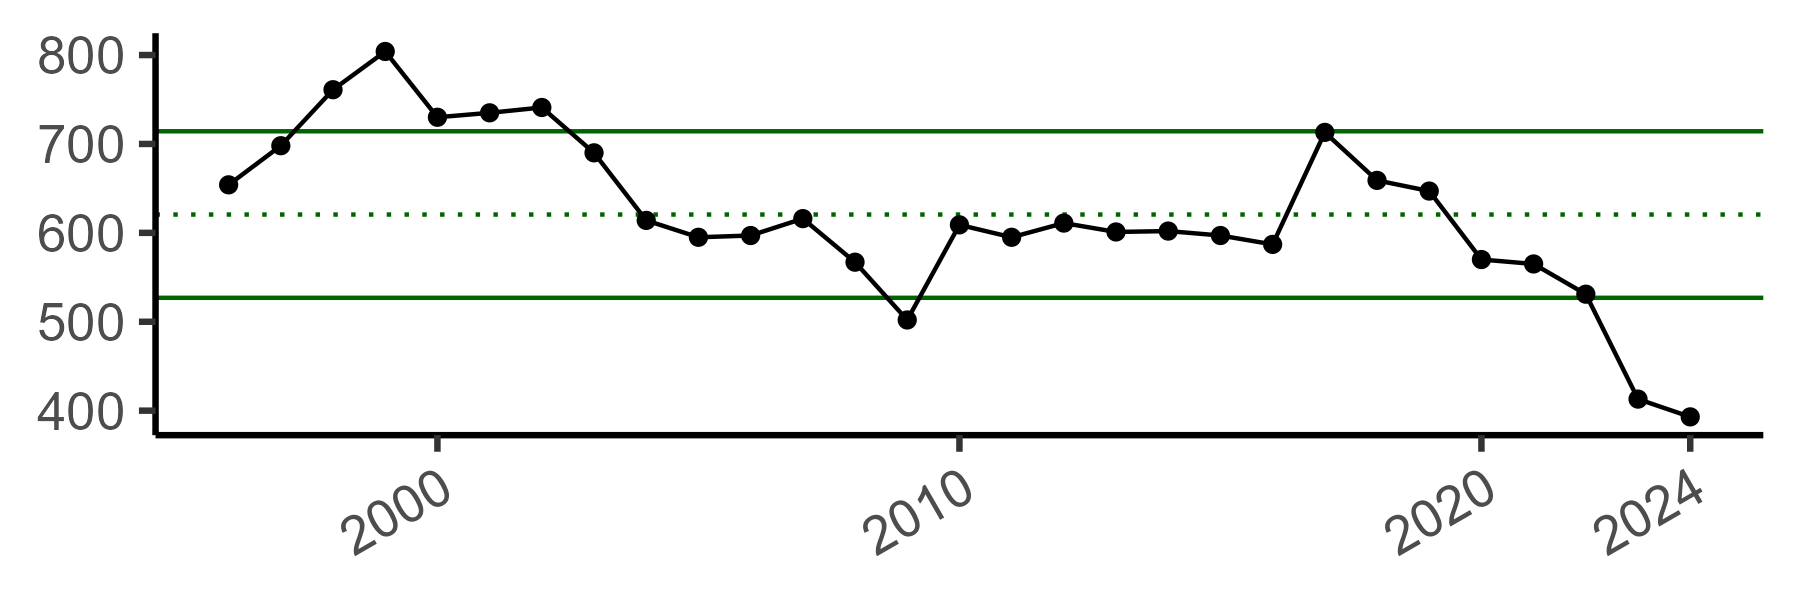
\includegraphics[width=3in, height=1in]{bsb_report_card_files/figure-pdf/unnamed-chunk-4-4.png}} \\

\ascline{0.75pt}{666666}{1-4}



\multicolumn{1}{!{\color[HTML]{666666}\vrule width 0.75pt}>{\raggedright}m{\dimexpr 0.9in+0\tabcolsep}}{\textcolor[HTML]{000000}{\fontsize{10}{10}\selectfont{\global\setmainfont{Times New Roman}{Number\ of\ commercial\ vessels\ (\#)}}}} & \multicolumn{1}{!{\color[HTML]{666666}\vrule width 0.75pt}>{\raggedright}m{\dimexpr 0.75in+0\tabcolsep}}{\textcolor[HTML]{000000}{\fontsize{10}{10}\selectfont{\global\setmainfont{Times New Roman}{Below\ long-term\ average}}}} & \multicolumn{1}{!{\color[HTML]{666666}\vrule width 0.75pt}>{\raggedright}m{\dimexpr 2.5in+0\tabcolsep}}{\textcolor[HTML]{000000}{\fontsize{10}{10}\selectfont{\global\setmainfont{Times New Roman}{The\ number\ of\ active\ vessels\ has\ been\ decreasing\ since\ 2017,\ which\ could\ impact\ revenue\ distributions\ and\ fleet\ composition. }}}} & \multicolumn{1}{!{\color[HTML]{666666}\vrule width 0.75pt}>{\centering}m{\dimexpr 3in+0\tabcolsep}!{\color[HTML]{666666}\vrule width 0.75pt}}{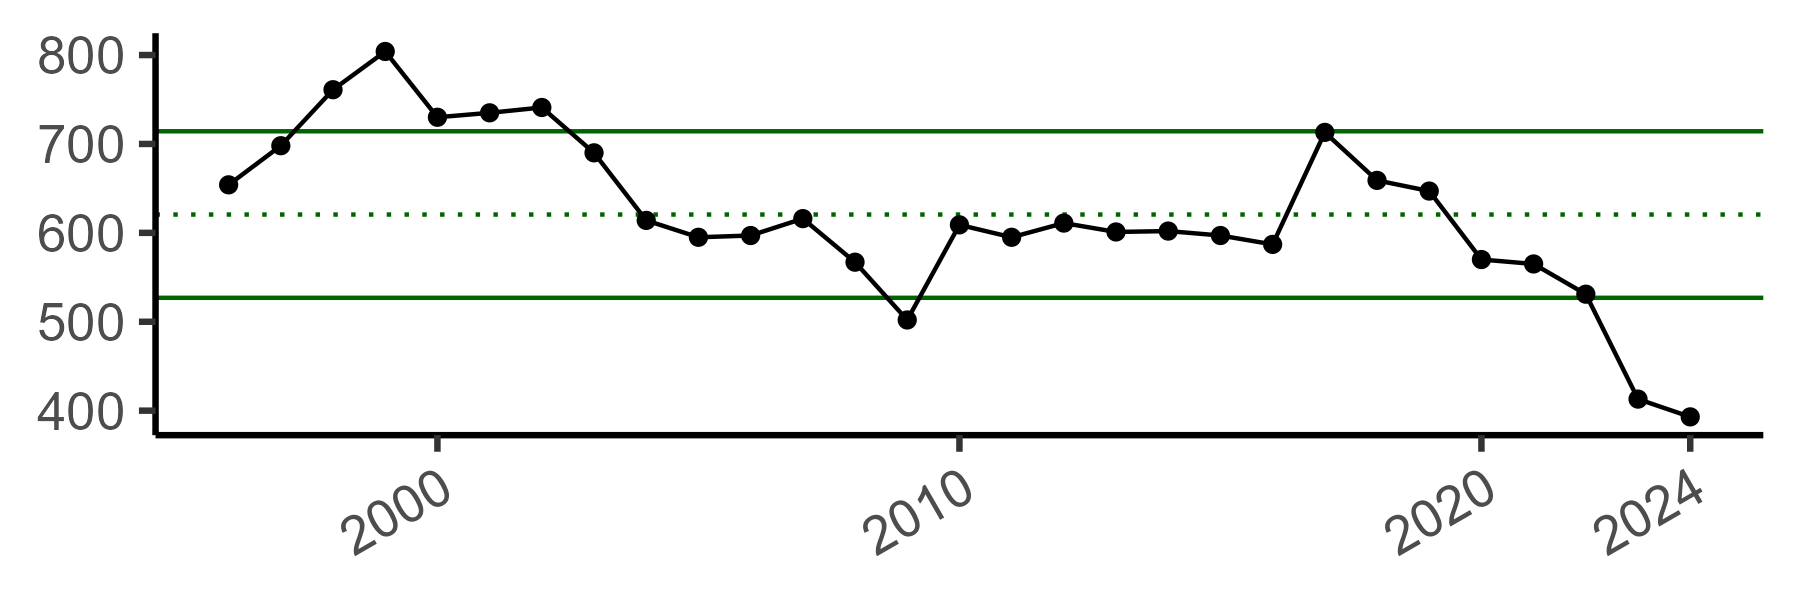
\includegraphics[width=3in, height=1in]{bsb_report_card_files/figure-pdf/unnamed-chunk-4-5.png}} \\

\ascline{0.75pt}{666666}{1-4}



\end{longtable*}



\arrayrulecolor[HTML]{000000}

\global\setlength{\arrayrulewidth}{\Oldarrayrulewidth}

\global\setlength{\tabcolsep}{\Oldtabcolsep}

\renewcommand*{\arraystretch}{1}

\vspace{-0.4cm}

\footnotesize * The y-axis units are included in the ``Indicator''
column of the table. In all figures, the dashed line represents the time
series mean, and the solid green lines indicate ± 1 standard deviation.
Commercial data were derived from the commercial dealer database hosted
at the Greater Atlantic Regional Office. All dollar values have been
adjusted to 2024 real dollars using the
\href{https://fred.stlouisfed.org/series/GDPDEF}{Gross Domestic Implicit
Price Deflator}.\newline\newline

\centering\normalsize

We welcome your observations! Please contact
northeast.ecosystem.highlights@noaa.gov with any on-the-water insights
or changes observed in the black sea bass fishery and
nefsc.esp.leads@noaa.gov with questions or comments on the information
presented in this report.

\newpage
\newgeometry{top=1in, left=1in, right=1in, bottom=1in}

\section{References}

\raggedright

Fratantoni, P.S., Holzworth-Davis, T., \& Taylor, M.H. (2015).
Description of oceanographic conditions on the Northeast US Continental
Shelf during 2014. US Dept Commer, Northeast Fisheries Science Center.
Ref Doc. 15-21; 41 p.~http://dx.doi.org/10.7289/V5SQ8XD2
\newline\newline

Jean-Michel, L., Eric, G., Romain, B.-B., Gilles, G., Angélique, M.,
Marie, D., Clément, B., Mathieu, H., Olivier, L. G., Charly, R., Tony,
C., Charles-Emmanuel, T., Florent, G., Giovanni, R., Mounir, B., Yann,
D., \& Pierre-Yves, L. T. (2021). The Copernicus Global 1/12° Oceanic
and Sea Ice GLORYS12 Reanalysis. Frontiers in Earth Science, 9, 698876.
https://doi.org/10.3389/feart.2021.698876 \newline\newline

MAFMC. (2024a). Black Sea Bass Fishery Information Document.
https://static1.squarespace.com/static/511cdc7fe4b00307a2628ac6/t/6683032fa306b9070227348b/1719862063436/2024\_BSB-fishery-info-doc.pdf
\newline\newline

MAFMC. (2024b). Summer Flounder, Scup, and Black Sea Bass Fishery
Performance Report.
https://static1.squarespace.com/static/511cdc7fe4b00307a2628ac6/t/6697d5dde4c39b20168045b7/1721226717179/b\_SFSBSB-FPR-Jul-2024.pdf
\newline\newline

MAFMC. (2024c). Summer Flounder, Scup, and Black Sea Bass Monitoring
Committee (MC) November 19, 2024 Webinar Meeting Summary 2025
Recreational Management Measures.
https://static1.squarespace.com/static/511cdc7fe4b00307a2628ac6/t/674755f846e791454569703f/1732728312681/01\_2025+SF+Rec+Measures.pdf
\newline\newline

MAFMC. (2024d). Mid-Atlantic EAFM Risk Assessment: 2024.
https://static1.squarespace.com/static/511cdc7fe4b00307a2628ac6/t/6747560a3cf66936045e5547/1732728332670/05\_EAFM+Risk+Assessment.pdf
\newline\newline

NEFSC. (2023). Report of the Black Sea Bass (Centropristis striata)
Research Track Stock Assessment Working Group.
https://d23h0vhsm26o6d.cloudfront.net/11a.-2023\_BSB\_UNIT\_RTWG\_Report\_V2\_12\_2\_2023.pdf
\newline\newline

Tabandera, R., Tyrell, A., McMahan, M., Perez, P., Hankowsky, K., \&
Large, S. (2024). Black sea bass ecosystem considerations and indicator
development. https://doi.org/10.25923/ez9g-af05



\end{document}
